\documentclass[a4,12pt]{scrartcl}

%Basic 
\usepackage[utf8]{inputenc}
\usepackage[ngerman]{babel}
\usepackage[T1]{fontenc}
%Schrift 
%\usepackage{fontspec} 
%\setmainfont{Arial} 
%Zeilenabstand
\usepackage{setspace}
\setstretch {1.3}
\usepackage{float}
\usepackage[bottom = 3.50cm]{geometry}

%Titel Seite
\usepackage{titling} %Wird benötigt damit \maketitle die Variabeln title, author und date nicht überschreibt
\title{Projektplan}
\subtitle{Projekt: software name}
\author{David Meister \and Andreas Stalder}		
 %mit /and können Personen hinzugefügt werden
\date{\today}


%Kopf, Fusszeile
\usepackage{fancyhdr}
\pagestyle{fancy}
\lhead{}
\chead{}
\rhead{software name}
\lfoot{\thetitle \: v1.0 }
\cfoot{\today }
\rfoot{Seite \thepage}
\renewcommand{\headrulewidth}{0.4pt}

%Bilder
\usepackage{graphicx}

%Zeichnen
\usepackage{tikz}

%Tabellen
\usepackage{booktabs}
\usepackage{longtable}

%Codesnippets
\usepackage{listings}
\lstset{language=java,basicstyle=\footnotesize,frame=single} %backgroundcolor=\color{lightgray}

%Querformat für eine Seite
\usepackage{lscape}
\usepackage{rotating}
\usepackage{pdflscape}

%URL 
\usepackage[colorlinks=true, linkcolor=blue, urlcolor=blue, citecolor=blue]{hyperref}
\urlstyle{same} 


%Loremimpsum
\usepackage{lipsum}



\begin{document}

%\clearpage\maketitle
\begin{titlepage}
	\centering
	\vspace{5cm}
	\begin{center}
%	\includegraphics[width=0.50\textwidth]{}
	\end{center}
	{\huge\bfseries software name\par}
	\vspace{8cm}
	\raggedright
	{\bfseries HSR Studienarbeit Network Unit Testing\par}
	{\huge\bfseries Projektplan\par}
	\vspace{1cm}
	{\theauthor \par}
	{\today\par}

\end{titlepage}

\section{Änderungsgeschichte}

\begin{table}[htb]
\centering
    \begin{tabular}{@{} l l l l@{}}\toprule    
    {Datum} & {Version} & {Änderung} & {Autor}\\ \midrule
    27.09.16 & 1.0 & Erstellung erster Version & dm/as\\ \addlinespace
    06.10.16 & 1.1 & Anpassung Iterationen \& Arbeitspakete & dm/as\\ \addlinespace
    \end{tabular}
\caption{\textbf{Änderungsgeschichte}}
\end{table}

\newpage

%\thispagestyle{empty}
\tableofcontents
\newpage


\section{Einführung}
\subsection{Zweck}
Dieses Dokument stellt den Projektplan für unser Studienarbeit dar, es dient zur Planung, Steuerung und Kontrolle.
\subsection{Gültigkeitsbereich}
Dieses Dokument ist über die gesamte Projektdauer gültig. Es wird in späteren Iterationen angepasst. Somit ist jeweils die neuste Version des Dokuments gültig und alte Versionen sind obsolet.
\subsection{Referenzen}
\begin{description}
Noch keine.
%  \item[jNetPcap] \hfill \\
%  \url{http://jnetpcap.com/}
\end{description}

\section{Projektübersicht}
Nach durchgeführten Changes im Netzwerkbereich wird die gewünschte Funktionalität meist von Hand getestet. In den meisten Fällen geschieht dies durch einfache Tools wie ping oder traceroute. Es wird vom durchführenden Netzwerk Engineer erwartet, dass er selbständig weiss, welche Funktionalität er nach durchgeführten Changes testen muss. Je nach Komplexität der Infrastruktur ist der Scope kaum in den Griff zu kriegen. \\

\noindent In der Software Entwicklung nutzt man schon lange Unit Tests. Optimalerweise werden für Softwareklassen zuerst Unit Tests geschrieben und anschliessend wird der Code implementiert. Somit existiert für jede Klasse und deren Methoden eine Testsammlung, welche bei späteren Changes immer ausgeführt werden kann. \\

\noindent Mit dieser Arbeit wird die Möglichkeit der Nutzung für Netzwerk Unit Tests angestrebt.
\subsection{Zweck und Ziel}
Die Studienarbeit soll den Nachweis der Problemlösungsfähigkeit unter Anwendung ingenieurmässiger Methoden nachweisen. Entsprechend verfügt die Arbeit über einen konzeptionellen, theoretischen und einen praktischen Anteil.\\

\noindent Mit Unit Tests für Netzwerkinfrastrukturen möchte man ein technisches Hilfsmittel für die Qualitätssicherung in der IT bereitstellen. Ähnlich wie in der Software Entwicklung soll eine Systematik entwickelt werden, um Komponenten im Netzwerk auf ihre Konfiguration und Funktionalität zu testen. 
\subsection{Lieferumfang}
noch nicht definiert
\subsection{Annahmen und Einschränkungen}
bisher noch keine Annahmen und Einschränkungen
\subsection{Organisationsstruktur}
\begin{table}[H]
\centering
    \begin{tabular}{@{} l l l l@{}}    
    {Vorname} & {Name} & {E-Mail} & Veratwortlich für\\ \midrule
    Andreas & Stalder & astalder@hsr.ch & -\\ \addlinespace
    David & Meister & dmeister@hsr.ch & -\\ \bottomrule
    \end{tabular}
\caption{\textbf{Teammitglieder}}
\end{table} 

\subsection{Externe Schnittstellen}
Das Projekt wird von Beat Stettler und Urs Baumann betreut und benotet.

\section{Management Abläufe}
\subsection{Zeitbudget}
Der Projektstart ist am Montag, dem 22. September 2016. \\
Die Projektdauer beträgt 14 Wochen, und das Projektende ist am Freitag, dem 23. Dezember 2016. \\

\noindent Während diesen 14 Wochen sind 240 Arbeitsstuden pro Projektmitglied eingeplant. Das entspricht pro Mitglied eine Arbeitszeit von ca. 18 Stunden pro Woche. Dies ergibt einen totalen Aufwand von ca. 480 Stunden.\\

\noindent Die wöchentliche Arbeitszeit von 18 Stunden kann bei Verzug oder bei unerwarteten Problemen auf maximal 24 Stunden erhöht werden. \\

\noindent Es sind gegenwärtig keine Absenzen während dieser Zeit geplant. 
\subsection{Zeitliche Planung}
Die Zeitplanung und die Verwaltung der Arbeitspakete erfolgt in Redmine. Diese wird während dem Projekt laufend aktualisiert. Die in Redmine erzeugten Tickets dienen sogleich als Arbeitspakete. Diese werden einer, ebenfalls im Redmine hinterlegten Iteration zugewiesen. Anhand von diesen Daten ist ein übersichtlicher Zeitplan ersichtlich. Um einen Überblick über den aktuellen Zeitplan zu erhalten, erfolgt der Zugriff auf das Gantt-Diagram via URL:
Die Projektmitglieder tragen jeweils die investierte Zeit am Abend in das zugewiesene Ticket ein. 

\subsubsection{Phasen}
Das Projekt wird in fünf Phasen unterteilt: Initialisierung, Analyse, Design, Realisierung und Abschluss.
\newline
\newline
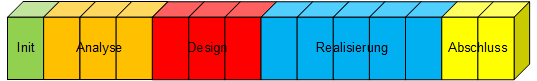
\includegraphics[width=1\textwidth]{figures/phasen.png}
\newpage

\subsubsection{Meilensteine}
Das Projekt beinhaltet insgesamt fünf Meilensteine. \\
\begin{table}[H]
    \begin{tabular}{@{} l l l r@{}}\toprule    
    {Meilenstein} & {Beschreibung} & {Datum}\\ \midrule
    MS1 & Anforderungen und Scope definiert  & 13.10.16\\ \addlinespace
    MS2 & Architektur und Design beschrieben & 03.11.16\\ \addlinespace
    MS3 & Betaversion fertiggestellt  & 24.11.16\\ \addlinespace
    MS4 & Software und Dokumentationen fertiggestellt  & 08.12.16\\ \addlinespace
    MS5 & Arbeitsabgabe & 23.12.16\\ 
    \bottomrule
    \end{tabular}
\caption{\textbf{Projekt Meilensteine}}
\end{table}


\subsubsection{Iterationen}
Die Dauer eines Iterationszyklus beträgt jeweils eine Woche. 
\begin{table}[htb]
\centering
    \begin{tabular}{@{} p{3cm} l l l@{}}\toprule    
    {Iteration} & {Inhalt} & {Start} & {Ende}\\ \midrule
    Initialisierung & Projektstart und Kickoff-Meeting & 15.09.2016 & 22.09.2016\\ \addlinespace
    Analyse 1 & Projektplanung & 23.09.2016 & 30.09.2016\\ \addlinespace
    Analyse 2 & Netzwerk Tests Analyse & 01.10.2016 & 06.10.2016\\ \addlinespace
    Analyse 3 & Requirements \& Evaluation & 07.10.2016 & 13.10.2016\\ \addlinespace
    Design 1 & - & 14.10.2016 & 20.10.2016\\ \addlinespace
    Design 2 & - & 21.10.2016 & 27.10.2016\\ \addlinespace
    Design 3 & - & 28.10.2016  & 03.11.2016\\ \addlinespace
    Realisierung 1 & - & 04.11.2016  & 10.11.2016\\ \addlinespace
    Realisierung 2 & - & 11.11.2016  & 17.11.2016\\ \addlinespace
    Realisierung 3 & - & 18.11.2016  & 24.11.2016\\ \addlinespace
    Realisierung 4 & - & 25.11.2016  & 01.12.2016\\ \addlinespace
    Realisierung 5 & - & 02.12.2016  & 08.12.2016\\ \addlinespace
    Abschluss 1 & - &  09.12.2016 & 15.12.2016\\ \addlinespace
    Abschluss 2 & - &  16.12.2016 & 23.12.2016\\ \addlinespace
    \bottomrule
    \end{tabular}
\caption{\textbf{Projekt Iterationen}}
\end{table}


\begin{landscape}
\subsubsection{Arbeitspakete (Tickets)}
\begin{longtable}{ p{5.5cm} p{8cm} l l p{1cm} p{1cm} }

\hline 
\multicolumn{1}{p{5.5cm}}{\textbf{Name}} & \multicolumn{1}{p{8cm}}{\textbf{Inhalt}} & \multicolumn{1}{l}{\textbf{Iteration}} & \multicolumn{1}{l}{\textbf{Wer}} & \multicolumn{1}{p{1cm}}{\textbf{Soll}} & \multicolumn{1}{p{1cm}}{\textbf{Ist}} \\ \hline 
\endfirsthead


\hline 
\multicolumn{1}{p{5.5cm}}{\textbf{Name}} & \multicolumn{1}{p{8cm}}{\textbf{Inhalt}} & \multicolumn{1}{l}{\textbf{Iteration}} & \multicolumn{1}{l}{\textbf{Wer}} & \multicolumn{1}{p{1cm}}{\textbf{Soll}} & \multicolumn{1}{p{1cm}}{\textbf{Ist}} \\ \hline 
\endhead


\textbf{Projektstart}&&&&\\ \addlinespace
Kickoff-Meeting & Allgemeine Besprechungen zum Projektstart & Initialisierung & Alle & 1 & 0.75 \\ \addlinespace
\textbf{Projektplanung}&&&&\\ \addlinespace
Projektübersicht & Projektübersicht verschaffen \& Kapitel im Projektplan erfassen & Analyse 1 & Alle & 8 & 6 \\
Zeitplanung & Projektphasen, Iterationen, Meilensteine definieren & Analyse 1 & alle & 5 & 6 \\
Risikomanagement & Projektrisiken abschätzen & Analyse 3 & alle & 8 & 0 \\
Qualitätsmanagement & Qualitätsmassnamen im Projekt definieren & Analyse 1& alle & 5 & 4 \\
\textbf{Netzwerk Tests Analyse}&&&&\\ \addlinespace
Einarbeitung & Recherche, Brainstorming, Diskussion & Analyse 1 \& 2& Alle & 10 & 15 \\ \addlinespace
Einleitung & Kapitel Einleitung & Analyse 2 & dm & 2 & 2 \\ \addlinespace
Device Tests & Recherche, Diskussion, Dokumentation & Analyse 2 & as & 4 & 3 \\ \addlinespace
Circuit Tests & Recherche, Diskussion, Dokumentation & Analyse 2 & dm & 4 & 7 \\ \addlinespace
Routing Tests & Recherche, Diskussion, Dokumentation & Analyse 2 & dm & 5 & 3 \\ \addlinespace
Traffic Tests & Recherche, Diskussion, Dokumentation & Analyse 2 & as & 4 & 3 \\ \addlinespace
Application Tests & Recherche, Diskussion, Dokumentation & Analyse 2 & as & 5 & 6 \\ \addlinespace
\textbf{Requirements}&&&&\\ \addlinespace
\textbf{Evaluation}&&&&\\ \addlinespace
 \addlinespace


\hline\caption{\textbf{Arbeitspakete}}
\end{longtable}
\end{landscape}




\subsection{Teammeetings}
Besprechungen finden wöchentlich jeweils am Dienstag statt. 
Eine Besprechung dauert in der Regel 30min und findet in der HSR statt. Bei einer Besprechung wird das weitere Vorgehen, sowie durchgeführte Arbeiten, fällige Arbeiten und auftretende Probleme besprochen. Weiter werden Arbeitspakete verteilt, damit beide Projektmitglieder wissen was zu tun ist. 

\subsubsection{Meeting mit Betreuern}
Die Meetings mit den Betreuern finden jeden Donnerstag um 13:30 Uhr statt. 
Die Meetings werden mit den Betreuern Beat Stettler und Urs Baumann in ihrem Büro durchgeführt. Die Dauer eines Meetings ist unterschiedlich und kann stark variieren. 

\section{Risikomanagement}
\subsection{Risiken}
Technische Risiken in der Entwicklung sind im Dokument TechnischeRisiken.xlsx aufgeführt.
\subsection{Umgang mit Risiken}
Die im Dokument TechnischeRisiken.xlsx aufgeführten Risiken sind in der Zeitplanung nicht speziell vorgesehen. Falls beim Eintreten eines geplanten Risikos ein erhöhter Zeitbedarf entsteht, so muss dies mit hoher Wahrscheinlichkeit mit Mehrarbeit der Teammitglieder kompensiert werden. Falls die nötige Mehrarbeit ausserhalb der Möglichkeiten liegt, so muss in Absprache aller Teammitglieder mit dem Betreuer nach einer anderer Lösung (z.B. Einschränkung von Programmfeatures, etc.) gesucht werden.


\section{Qualitätsmassnahmen}

\subsection{Dokumentation}
Alle Datein, welche Teil der Dokumentation sind, werden mit git versioniert. Das git Repository befindet sich auf GitHub.
\subsection{Projektmanagement}
Als Projektmanagementsoftware wird Redmine eingesetzt. 
Es wird nach jeder Arbeitssession oder beim Wechsel einer Arbeit der Aufwand auf das entsprechende Ticket verbucht.
Zugriff auf Redmine erfolg über die Url: - % TODO: noch erfassen}
Um den Zugriff für Betreuungspersonen zu ermöglichen wurde ein Gastbenutzer eingerichtet.
\newline
\newline
Logindaten Redmine Gastbenutzer:
\begin{description}
\begin{description}
\item [Login:]
-
% TODO: Login erfassen
\item [Password:]
-
% TODO: Login erfassen
\end{description}
\end{description}


\subsection{Entwicklung}

\subsubsection{Versionierung}
Wie die Dokumentation wird auch der Sourcecode mit git versioniert und auf GitHub abgelegt. Es wird darauf geachtet, möglichst häufig auf den Stamm zu commiten.
\subsubsection{Test Driven Development}
Es hat sich herausgestellt, dass die Software Qualität mit Test Driven Development (TDD) am besten ist. Beim TDD wird vor der Implementation der dazugehörige Unit Test entwickelt. Wo überall möglich, wird mittels TDD entwickelt.
\subsubsection{Reviews}
Regelmässige Reviews sind in einem iterativen Vorgehen unerlässlich. Die getätigte Arbeit muss ständig abgeglichen und in Frage gestellt werden. Aus Kosten-Nutzen Sicht sind Reviews das effektivste Mittel um die geforderte Qualität zu erreichen.\\ 

\noindent In diesem Projekt werden drei verschiedene Arten von Reviews durchgeführt. Zum einen sind dies regelmässige Code Reviews, zum anderen sind dies Requirement- und Architekturreviews.\\

\noindent Bei den regelmässigen Code Reviews wird besonders auf die gewählten Namen (Packages, Klassen, Methoden, Variablen), die Verständlichkeit vom Code und Code Smells geachtet.\\

\noindent Bei den Requirement Reviews wird sichergestellt, dass man den Wünschen des Auftraggebers entsprechend entwickelt. Die Frage nach dem "Was" wird erneut gestellt und somit sichergestellt, dass man beim Projektende nicht ein qualitativ hochwertiges Produkt entwickelt hat, welches aber nicht die Wünsche des Auftraggebers abdeckt.\\ 

\noindent Beim Architektur Review wird besonders auf die nicht-funktionalen Anforderungen (NFA) geachtet. Diese wirken sich in den meisten Fällen auf die gewählte Architektur aus. Die gewählte Architektur muss mit den NFA's verträglich sein. Wenn zu spät im Projekt bemerkt wird, dass die Architektur geändert werden muss, kann dies sehr aufwändig sein.
\subsubsection{Code Metriken}
Code Metriken zeigen mögliche Fehler oder Schwachstellen im entwickelten Code auf. Es wird grundsätzlich zwischen statischen- und dynamischen Metrik Tools unterschieden. Bei den dynamischen Metrik Tools wird der Code ausgeführt. Beispiele wären Unit Tests und die dazugehörige Coverage. Bei den statischen Analysetools wird der Code nicht ausgeführt. Ein Beispiel wäre Checkstyle. Dieses Tool überprüft vor allem die Einhaltung von Style Richtlinien.\\

\noindent Um diese mächtigen Tools effektiv nutzen zu können, müssen sie in den Build Prozess mit eingebunden werden. SonarQube stellt ein Modul für Build-Management-Tools bereit, sodass statische Code Analysen automatisch beim Build ausgeführt werden.
\subsubsection{Continuous Integration}
Mittels Continuous Integration (CI) wird das Risiko von schleichenden Softwarebugs minimiert. Jeder commit in den Stamm triggert einen kompletten Build der Software auf dem CI-Server. Somit wird immer ersichtlich, falls Fehler im Build auftauchen oder Unit Tests fehlschlagen.\\

\noindent Als CI-Server wird Jenkins verwendet. Jenkins ist frei verfügbar und bietet nebst guter cross-platform Unterstützung mächtige Tools zur automatischen Überprüfung mittels statischen Code Analyse Tools.

\end{document}

